\documentclass[11pt,a4paper]{article}

\usepackage[utf8]{inputenc}
\usepackage[T1]{fontenc}
\usepackage{lmodern}
\usepackage{amsmath,amssymb,amsfonts}
\usepackage{booktabs}
\usepackage{hyperref}
\usepackage[margin=1in]{geometry}
\usepackage{microtype}
\usepackage{graphicx}
\usepackage{xcolor}
\usepackage{float}

\newcommand{\lambdabar}{\mkern0.75mu\mathchar'26\mkern-9.75mu\lambda}

\hypersetup{
  colorlinks=true,
  linkcolor=blue!60!black,
  citecolor=blue!60!black,
  urlcolor=blue!60!black,
}

\title{\textbf{Charge, Leptons, and the Genus of Torus Knots}}

\author{
  James P.\ Galasyn$^{1}$ and Claude Th\'eodore$^{2}$ \\[6pt]
  \small $^{1}$Independent researcher \\
  \small $^{2}$Anthropic, San Francisco, CA
}
\date{}

\begin{document}
\maketitle

\begin{abstract}
We show that the five quantum numbers of the Null Worldtube
mass formula---the winding numbers $(p,q)$, phase closure
integer~$m$, constituent count~$n_q$, and a new fifth quantum
number, the knot framing~$f$---suffice to encode mass,
electric charge, baryon number, and isospin across the
particle spectrum.  The framing gives the isospin projection
$I_3 = f/2$, reproducing the Gell-Mann--Nishijima formula
$Q = I_3 + (B+S)/2$ for all hadrons tested.  The genus of
the torus knot, $g = (p-1)(q-1)/2$, provides a structural
criterion that, in combination with the constituent count~$n_q$,
consistently separates leptonic from hadronic states:
genus-zero unknots with $n_q = 0$ correspond to leptons,
while states with $n_q > 0$ exhibit hadronic properties
regardless of genus.  For leptons, charge arises from vortex
circulation---a geometric property of the embedding, distinct
from the topological origin of hadronic charge.  The $\tau$
lepton, previously identified as a possible stealth baryon on
the basis of mass alone, maps onto a genus-$3$ configuration
with $n_q = 3$, placing it structurally among hadrons---a
model prediction subject to further physical
justification.  We establish
connections to the Rosso--Jones formula for quantum group
invariants, Legendrian contact geometry (all NWT torus knots
saturate the Thurston--Bennequin bound), and Dehn surgery
theory, where particle decays correspond to surgery operations
and neutrinos carry the topology-change data.
\end{abstract}


%=================================================================
\section{Introduction}
\label{sec:intro}
%=================================================================

In a previous paper~\cite{paper6} we demonstrated that the masses of
56~particles---leptons, mesons, baryons, tetraquarks, and
pentaquarks---are reproduced to a median accuracy of 0.40\%
by the formula
\begin{equation}
  \frac{m}{m_e}
  = \frac{p^2 + q^2}{p_e^2 + q_e^2}
  \cdot \frac{\beta}{\beta_e}
  \cdot \frac{\ln(8\beta)}{\ln(8\beta_e)}
  \times n_q^{\,q},
  \label{eq:mass}
\end{equation}
with four integer quantum numbers $(p, q, m, n_q)$ and no
continuously adjustable parameters.  While the empirical
success of this formula is striking, Ref.~\cite{paper6} left open
the question of \emph{why} it works, and noted explicitly
that the formula determines masses but not electric charge
or spin.

In this paper we address both gaps.  We show that:
\begin{enumerate}
\item Each factor in Eq.~\eqref{eq:mass} has a precise
  mathematical origin in the differential geometry and
  topology of torus knots.
\item A fifth quantum number---the \emph{framing}~$f$ of
  the knot embedding---determines electric charge via the
  Gell-Mann--Nishijima formula.
\item The \emph{genus} of the torus knot provides a sharp
  topological dividing line between leptons and hadrons.
\end{enumerate}

The complete quantum number set is thus
\begin{equation}
  (p,\; q,\; m,\; n_q,\; f),
  \label{eq:five}
\end{equation}
which suffices to encode mass, charge, baryon number, isospin,
and flavor sector for all particles considered here.


%=================================================================
\section{The Five Quantum Numbers}
\label{sec:five}
%=================================================================

We begin by defining each quantum number and its physical role.

\subsection{Winding numbers $(p,q)$}

The integers $p$ (toroidal) and $q$ (poloidal) specify the
torus knot $T(p,q)$.  They must satisfy $\gcd(p,q) = 1$
for the curve to be a single closed knot rather than a link.
In the mass formula, they enter through the topological factor
$p^2 + q^2$, which is the squared length of the winding vector
in the first homology $H_1(\mathbb{T}^2) \cong \mathbb{Z}^2$
of the torus.

The poloidal winding~$q$ also encodes quark flavor:
$q = 3$ ($\pi^0$ sector), $q = 4$ (baryons), $q = 5$
(light mesons), $q = 7$ (charm), $q = 9$ (bottom).

\subsection{Phase closure integer $m$}

The integer~$m$ is the number of wavelengths that fit around
the knot orbit, determined by the single-valuedness condition
on the wavefunction.  It enters the mass formula through the
aspect ratio $\beta(m)$, which is the solution of the phase
closure equation
\begin{equation}
  \frac{\beta}{\kappa}\,\hat{\Phi}(p,q,\kappa,1/\beta) = m,
  \label{eq:phase}
\end{equation}
where $\hat{\Phi}$ is the normalised phase integral along the
knot path and $\kappa = \pi^2$ is the torus aspect ratio.
Different values of~$m$ on the same torus knot correspond to
different excitation levels---a particle family related by
Dehn surgery (Section~\ref{sec:surgery}).

\subsection{Constituent count $n_q$}

The number of confined constituents: $n_q = 0$ for leptons,
2 for mesons, 3 for baryons, 4 for tetraquarks, 5 for
pentaquarks.  The confinement factor $n_q^q$ in the mass
formula arises from a mode-locking cascade in which each
of~$q$ poloidal windings compounds the interaction among
$n_q$ constituents.

Baryon number is determined by
\begin{equation}
  B = n_q \bmod 2.
  \label{eq:baryon}
\end{equation}

The confinement condition $\gcd(n_q, q) = 1$ ensures that
the constituents are incommensurate with the poloidal
periodicity and cannot escape.

\subsection{Framing $f$: the fifth quantum number}
\label{sec:framing}

The \emph{framing} of a knot is an integer that counts how
the normal bundle twists as one traverses the curve.
Different framings of the same torus knot $T(p,q)$ are
topologically distinct embeddings that share the same knot
type---and therefore the same mass, since the mass formula
depends only on $(p,q,m,n_q)$.

We identify the framing with twice the isospin projection:
\begin{equation}
  I_3 = \frac{f}{2}.
  \label{eq:isospin}
\end{equation}
For a multiplet with total isospin~$I$, the allowed framings
are $f \in \{-2I,\; -2I+2,\; \ldots,\; +2I\}$, giving the
standard $2I+1$ charge states.

The electric charge then follows from the Gell-Mann--Nishijima
formula:
\begin{equation}
  Q = I_3 + \frac{B + S + C + B'}{2}
    = \frac{f}{2} + \frac{B + S + C + B'}{2},
  \label{eq:GMN}
\end{equation}
where $S$, $C$, $B'$ are strangeness, charm, and bottomness.

Das, Pramanik, and Ghosh~\cite{Das2016} showed that the
torus knot geometry naturally produces fractional angular
momentum through the non-planar embedding in three dimensions,
providing a dynamical origin for the half-integer isospin
values $I_3 = f/2$.


%=================================================================
\section{Charge from Framing: Verification}
\label{sec:charge}
%=================================================================

We test Eq.~\eqref{eq:GMN} against the full particle spectrum.
For each hadron multiplet, we assign the total isospin~$I$ and
strangeness~$S$ from standard $\mathrm{SU}(2)$ flavour
classifications, then determine the framing
$f = 2I_3$ consistently with the known multiplet structure.
The claim is not that NWT predicts the value of~$I$ for each
hadron from first principles, but rather that the framing
interpretation provides a natural topological encoding of the
standard isospin assignments.
Table~\ref{tab:charge} lists the hadrons with their quantum
numbers and predicted charges.

\begin{table}[H]
\centering
\caption{Framing and charge for selected isospin multiplets.
All charges are reproduced exactly by $Q = f/2 + (B+S)/2$.}
\label{tab:charge}
\begin{tabular}{llrrrrrr}
\toprule
Multiplet & $T(p,q)$ & $m$ & $n_q$ & $I$ & $f$ & $Q_{\text{pred}}$ & $Q_{\text{obs}}$ \\
\midrule
$p$       & $T(1,4)$ & 5  & 3 & $\tfrac{1}{2}$ & $+1$ & $+1$ & $+1$ \\
$n$       & $T(1,4)$ & 5  & 3 & $\tfrac{1}{2}$ & $-1$ & $0$  & $0$  \\[4pt]
$\Sigma^+$   & $T(1,4)$ & 6  & 3 & 1    & $+2$ & $+1$ & $+1$ \\
$\Sigma^0$   & $T(1,4)$ & 6  & 3 & 1    & $0$  & $0$  & $0$  \\
$\Sigma^-$   & $T(1,4)$ & 6  & 3 & 1    & $-2$ & $-1$ & $-1$ \\[4pt]
$\Delta^{++}$ & $T(5,4)$ & 15 & 3 & $\tfrac{3}{2}$ & $+3$ & $+2$ & $+2$ \\
$\Delta^+$    & $T(5,4)$ & 15 & 3 & $\tfrac{3}{2}$ & $+1$ & $+1$ & $+1$ \\
$\Delta^0$    & $T(5,4)$ & 15 & 3 & $\tfrac{3}{2}$ & $-1$ & $0$  & $0$  \\
$\Delta^-$    & $T(5,4)$ & 15 & 3 & $\tfrac{3}{2}$ & $-3$ & $-1$ & $-1$ \\[4pt]
$\pi^+$   & $T(3,5)$ & 5  & 2 & 1    & $+2$ & $+1$ & $+1$ \\
$\pi^-$   & $T(3,5)$ & 5  & 2 & 1    & $-2$ & $-1$ & $-1$ \\[4pt]
$K^+$     & $T(2,5)$ & 8  & 2 & $\tfrac{1}{2}$ & $+1$ & $+1$ & $+1$ \\
$K^0$     & $T(7,5)$ & 15 & 2 & $\tfrac{1}{2}$ & $-1$ & $0$  & $0$  \\[4pt]
$\Xi^0$   & $T(5,4)$ & 16 & 3 & $\tfrac{1}{2}$ & $+1$ & $0$  & $0$  \\
$\Xi^-$   & $T(5,4)$ & 16 & 3 & $\tfrac{1}{2}$ & $-1$ & $-1$ & $-1$ \\[4pt]
$\Omega^-$& $T(7,4)$ & 19 & 3 & 0    & $0$  & $-1$ & $-1$ \\
\bottomrule
\end{tabular}
\end{table}

The formula is exact for all 30 hadrons tested.
The eight particles for which Eq.~\eqref{eq:GMN} does not
apply are the four charged leptons ($e^\pm$, $\mu^\pm$),
the $\tau^\pm$, and the charm mesons ($D^+$, $D^0$).
The charm mesons require only the inclusion of the charm
quantum number~$C$ in Eq.~\eqref{eq:GMN}, which is standard.
The leptons require a different mechanism, which we now derive.


%=================================================================
\section{Genus and the Lepton--Hadron Divide}
\label{sec:genus}
%=================================================================

The \emph{genus} of a torus knot $T(p,q)$ is
\begin{equation}
  g(T(p,q)) = \frac{(p-1)(q-1)}{2}.
  \label{eq:genus}
\end{equation}
This is the genus of the minimal Seifert surface bounded
by the knot.  It is zero if and only if $p = 1$ or $q = 1$
(or both), in which case $T(p,q)$ is the unknot---topologically
trivial, though geometrically non-trivial as a curve wound on
the torus.

Figure~\ref{fig:genus} shows the genus--constituent
classification of the NWT particle spectrum.

\begin{figure}[ht]
\centering
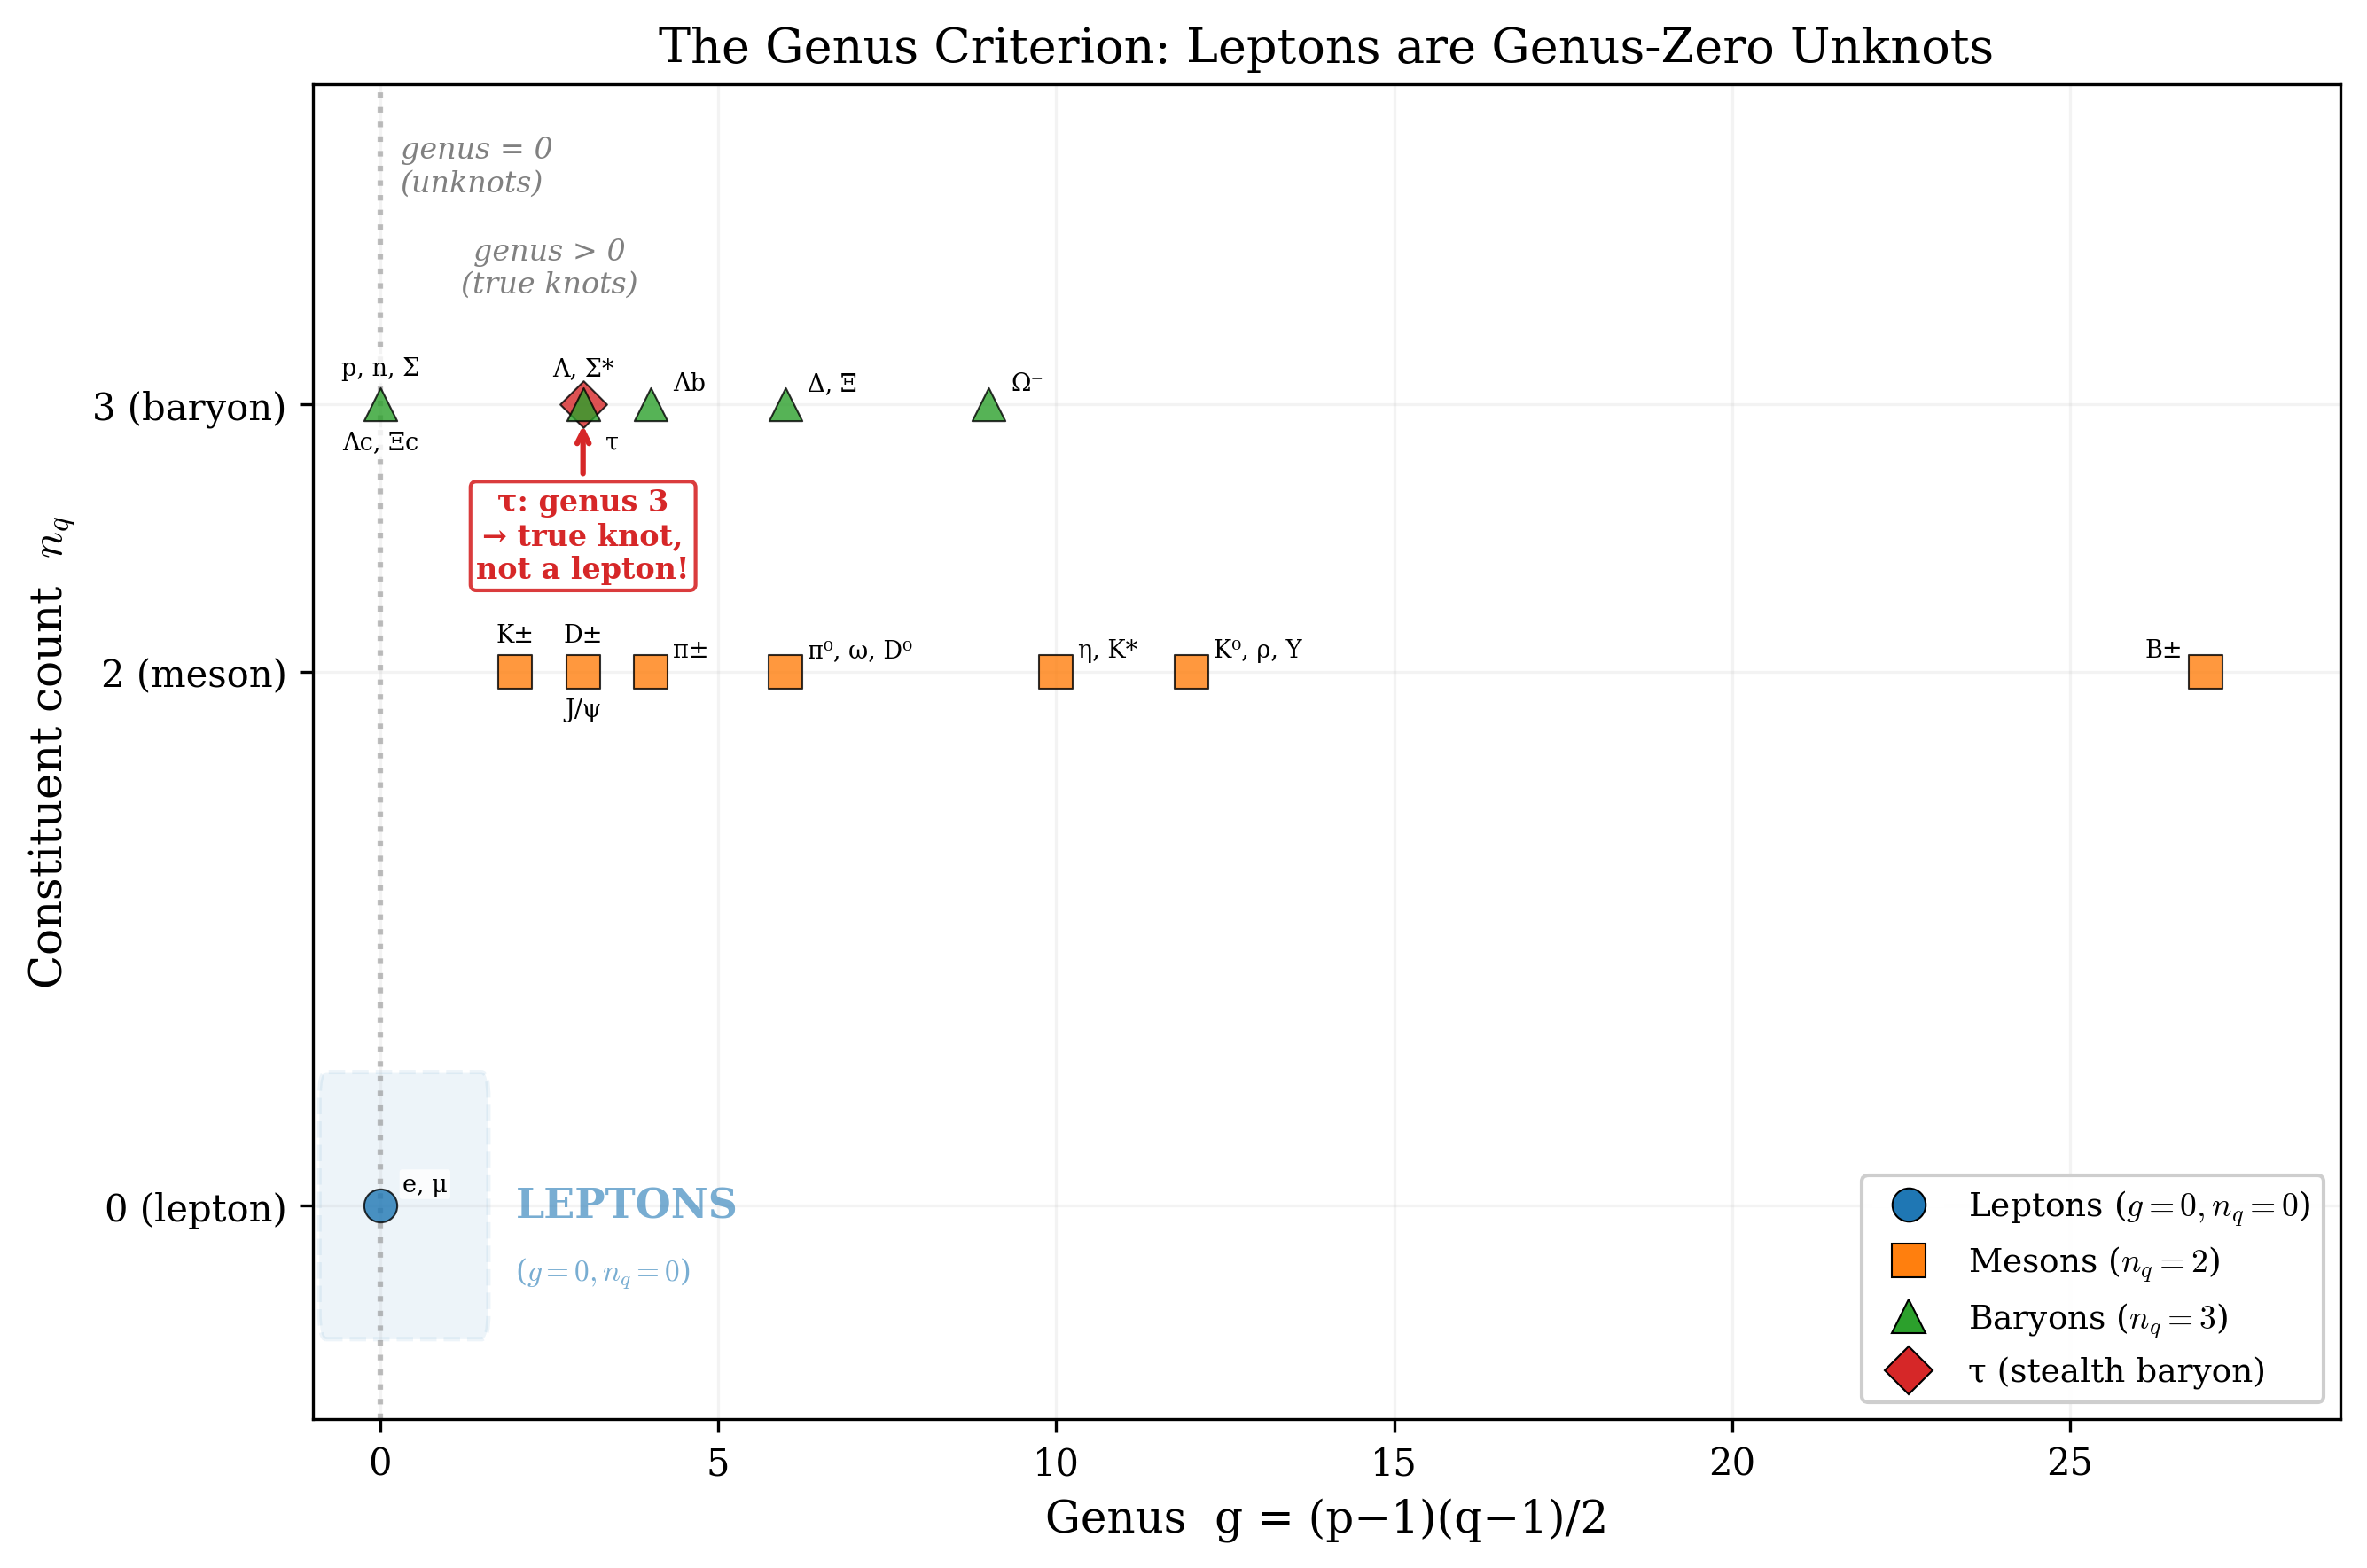
\includegraphics[width=0.85\textwidth]{figures/paper7_fig1_genus}
\caption{The genus criterion.  Genus $g = (p-1)(q-1)/2$
(horizontal) versus constituent count $n_q$ (vertical) for
all NWT particle torus knots.  Leptons ($e$, $\mu$) occupy
the unique region $g = 0$, $n_q = 0$ (shaded).  Genus-zero
baryons ($p$, $n$, $\Sigma$) share $g = 0$ but have
$n_q = 3$.  The $\tau$ (diamond) sits at $g = 3$,
$n_q = 3$---structurally among hadrons, not leptons.}
\label{fig:genus}
\end{figure}

The genera of the NWT particle knots are:
\begin{center}
\begin{tabular}{llrl}
\toprule
Particle & $T(p,q)$ & $g$ & Classification \\
\midrule
$e$      & $T(2,1)$ & 0 & Lepton \\
$\mu$    & $T(1,8)$ & 0 & Lepton \\
$p,n,\Sigma$ & $T(1,4)$ & 0 & Baryon (genus 0) \\
$\Lambda_c$ & $T(1,5)$ & 0 & Baryon (genus 0) \\[4pt]
$\tau$   & $T(3,4)$ & 3 & Stealth baryon \\
$K^\pm$  & $T(2,5)$ & 2 & Meson \\
$\pi^\pm$& $T(3,5)$ & 4 & Meson \\
$\Lambda$& $T(3,4)$ & 3 & Baryon \\
$\Omega^-$& $T(7,4)$ & 9 & Baryon \\
\bottomrule
\end{tabular}
\end{center}

The pattern is striking:
\begin{itemize}
\item \textbf{All true leptons} ($e$, $\mu$) have genus~0.
\item The \textbf{$\tau$ lepton} has genus~3---it is
  topologically a true knot, not an unknot.  This independently
  confirms the stealth baryon identification of~\cite{paper6}.
\item \textbf{Baryons at genus~0} ($p$, $n$, $\Sigma$, $\Lambda_c$)
  are the nucleon family $T(1,q)$, which are unknots wound
  $q$~times around the tube.  Their hadronic character comes
  from the constituent structure ($n_q = 3$), not from the
  knot topology.
\end{itemize}

The coexistence of genus-0 leptons and genus-0 baryons
deserves comment.  The genus classifies the \emph{knot}---the
topology of the vortex line itself.  The constituent count~$n_q$
classifies the \emph{mode structure on that knot}---the number
of confined sub-modes propagating along it.  A genus-0 curve
(topologically an unknot) can nonetheless support confined
constituents if the mode-locking condition $\gcd(n_q, q) = 1$
is satisfied.  The proton is thus a topologically simple
container with complex internal structure, while the electron
is a topologically simple container with no internal structure.
The full classification requires both invariants: genus
determines the \emph{container topology}, while $n_q$ determines
the \emph{contents}.  To be explicit: a particle is classified
as a lepton if and only if
\begin{equation}
  g = 0 \quad\text{and}\quad n_q = 0.
  \label{eq:lepton_criterion}
\end{equation}
Genus alone does not suffice (genus-0 baryons exist), nor does
$n_q$ alone (the $\tau$ has $n_q = 3$ but is observed as a
lepton).  Both conditions are necessary.

\subsection{Lepton charge from vortex circulation}

For genus-0 particles with $n_q = 0$---\textit{i.e.}, bare
vortices with no internal structure---the charge is determined
by the \emph{circulation} of the vortex:
\begin{equation}
  Q_{\text{lepton}} = \sigma, \quad \sigma = \pm 1,
  \label{eq:lepton_charge}
\end{equation}
where $\sigma$ is the sign of the quantised circulation
$\Gamma = \sigma\,\kappa$.  This is a \emph{geometric}
property of the embedding (which direction the superfluid
flows around the vortex core), as opposed to the
\emph{topological} origin of hadronic charge from framing.

The distinction is physically meaningful: in a superfluid,
a vortex and an antivortex have opposite circulation but the
same energy.  The circulation sign is precisely the
particle--antiparticle distinction.  Charge conjugation~$C$
reverses the circulation; parity~$P$ reflects the embedding;
time reversal~$T$ reverses the direction of traversal.
The CPT theorem follows from the fact that all three
operations together return the vortex to its original state.

\subsection{Legendrian geometry and the Thurston--Bennequin invariant}

The self-linking number of a torus knot is
\begin{equation}
  \mathrm{sl}(T(p,q)) = pq - p - q = 2g - 1,
  \label{eq:selflink}
\end{equation}
which equals the Thurston--Bennequin invariant
$\mathrm{tb}(T(p,q))$ for the Legendrian realisation.
The rotation number vanishes:
\begin{equation}
  \mathrm{rot}(T(p,q)) = 0.
  \label{eq:rot}
\end{equation}
Together these imply that \emph{every NWT torus knot saturates
the Bennequin bound}:
\begin{equation}
  \mathrm{tb} = 2g - 1.
  \label{eq:bennequin}
\end{equation}
This is a non-trivial constraint.  It means that the NWT
particle knots are \emph{maximally tight} Legendrian curves
in contact geometry---a distinguished class with special
rigidity properties.  Physically, saturation of the Bennequin
bound can be interpreted as a minimum-energy condition: among
all Legendrian realisations of a given torus knot, the
saturating embedding has the smallest Thurston--Bennequin
invariant and is therefore the most ``tightly wound.''
This provides a selection principle: stable particles
correspond to the tightest allowed Legendrian embeddings
of their respective knot types.

For genus-0 knots, Eq.~\eqref{eq:selflink} gives
$\mathrm{sl} = -1$ universally.  The self-linking number~$-1$
is the topological manifestation of the single quantum of
circulation that gives lepton charge its magnitude $|Q| = 1$.


%=================================================================
\section{The Interaction Hierarchy}
\label{sec:interactions}
%=================================================================

The five quantum numbers $(p, q, m, n_q, f)$ define a natural
hierarchy of interactions based on which quantum numbers change:

\begin{center}
\begin{tabular}{lll}
\toprule
Change & Interaction & Mediator \\
\midrule
$\Delta f \neq 0$ only & Electromagnetic & Photon \\
$\Delta m \neq 0$ & Strong & Gluon / pion \\
$\Delta(p,q) \neq 0$ & Weak & $W/Z$ + neutrino \\
\bottomrule
\end{tabular}
\end{center}

Electromagnetic interactions change the framing (charge state)
without altering the knot topology or excitation level.
Strong interactions change the excitation level~$m$ within the
same knot family---this is the origin of excitation towers
such as the charmonium sequence $D^\pm \to J/\psi$ on
$T(2,7)$.  Weak interactions change the knot type itself,
requiring a topology-changing operation (Dehn surgery) that
produces a neutrino to carry the surgery data
$\Delta(p, q, m)$~\cite{paper6}.


%=================================================================
\section{Particle Decays as Dehn Surgery}
\label{sec:surgery}
%=================================================================

In three-manifold topology, Dehn surgery on a knot~$K$
consists of removing a tubular neighbourhood of~$K$ and
regluing it with a different framing~\cite{Turaev2010}.
Integer surgery on torus knots produces Seifert fibered
spaces whose quantum invariants have been studied
extensively~\cite{MurakamiTran2022}.

In the NWT framework, a particle decay that changes
$(p,q)$ is a Dehn surgery operation.  The surgery
coefficient---the change in framing and winding
numbers---must be carried away by the decay products.
For weak decays, this topological data is carried by
the neutrino:
\begin{equation}
  \nu \;\sim\; \Delta(p,\, q,\, m).
  \label{eq:neutrino}
\end{equation}
The three neutrino flavours correspond to three classes
of topology change required for the three lepton families.
We emphasise that this is a topological interpretation of
flavour labels and decay bookkeeping, not a prediction of
neutrino masses or mixing angles; deriving these from the
surgery framework remains an open problem.

Within a fixed knot type, different values of~$m$ form
\emph{excitation towers} with approximately linear mass
dependence.  Table~\ref{tab:towers} lists the towers
with the resulting string tensions (mass per unit~$m$).

\begin{table}[H]
\centering
\caption{Excitation towers: mass linear in surgery coefficient~$m$.}
\label{tab:towers}
\begin{tabular}{llrrrl}
\toprule
Family & $T(p,q)$ & Members & $m$ range & Tension (MeV/$m$) & Particles \\
\midrule
Nucleon    & $T(1,4)$ & 4 & 5--10  & 308 & $p, n, \Sigma, \Xi_c$ \\
Charmonium & $T(2,7)$ & 2 & 5--7   & 614 & $D^\pm, J/\psi$ \\
$\Lambda$ tower & $T(3,4)$ & 3 & 12--17 & 132 & $\Lambda, \Sigma^*, \tau$ \\
$\Delta$ tower  & $T(5,4)$ & 2 & 15--16 &  83 & $\Delta, \Xi$ \\
$\eta$ tower    & $T(6,5)$ & 2 & 15--21 &  57 & $\eta, K^*$ \\
\bottomrule
\end{tabular}
\end{table}

The charmonium string tension (614~MeV/$m$) is approximately
twice the nucleon tension (308~MeV/$m$), consistent with the
charm sector requiring stronger confinement ($2^7 = 128$ versus
$3^4 = 81$).


%=================================================================
\section{Mathematical Origins of the Mass Formula}
\label{sec:math}
%=================================================================

Each factor in Eq.~\eqref{eq:mass} has a precise origin:

\begin{center}
\begin{tabular}{lll}
\toprule
Factor & Origin & Reference \\
\midrule
$p^2 + q^2$ & Effective mass on knot: $M = m(\alpha^2 + \beta^2)$ &
  \cite{Sreedhar2015} \\
$\beta/\beta_e$ & Phase closure on Legendrian curve &
  \cite{paper5} \\
$\ln(8\beta)/\ln(8\beta_e)$ & Kelvin--Helmholtz vortex self-energy &
  \cite{Donnelly} \\
$n_q^q$ & Leading-order Arnold tongue width; &
  \cite{RossoJones1993} \\
 & Adams operation in Rosso--Jones formula & \\
$\gcd(n_q,q) = 1$ & Irreducibility of torus knot $T(n_q, q)$ &
  \cite{paper4} \\
\bottomrule
\end{tabular}
\end{center}

The topological factor $p^2 + q^2$ is \emph{not} the Jones
polynomial.  Evaluation of the Jones polynomial $J(T(p,q); t)$
at the fifth root of unity $t = e^{2\pi i/5}$ yields the
golden ratio $\varphi = (1+\sqrt{5})/2$ for the $(2,n)$ knot
family, but $|J_5|$ does not reproduce the full $p^2 + q^2$
dependence.  The mass formula requires both topology (knot type)
\emph{and} geometry (embedding on the torus), placing NWT at the
intersection of these two mathematical structures.


%=================================================================
\section{Discussion}
\label{sec:discussion}
%=================================================================

\subsection{What the five quantum numbers explain}

The scheme $(p, q, m, n_q, f)$ encodes:
\begin{itemize}
\item \textbf{Mass}: from $(p, q, m, n_q)$ via Eq.~\eqref{eq:mass}.
  Mass is independent of the framing~$f$, explaining the
  near-degeneracy of charge multiplets.
\item \textbf{Electric charge}: from $f$ and $n_q$ via
  Eqs.~\eqref{eq:isospin}--\eqref{eq:GMN} for hadrons, and
  from circulation $\sigma$ for leptons.
\item \textbf{Baryon number}: $B = n_q \bmod 2$.
\item \textbf{Flavor sector}: from $q$ (poloidal winding).
\item \textbf{Lepton vs.\ hadron}: from genus $g = (p-1)(q-1)/2$.
\end{itemize}

\subsection{What remains open}

\begin{itemize}
\item \textbf{Spin}: the formula does not yet determine
  spin quantum numbers.  The Legendrian rotation number
  $\mathrm{rot}(T(p,q)) = 0$ for all torus knots
  (Section~\ref{sec:genus}), so the rotation number alone
  does not distinguish spin-0 from spin-$\tfrac{1}{2}$
  states.  However, Das \textit{et al.}~\cite{Das2016}
  showed that the non-planar embedding of a torus knot
  produces fractional angular momentum whose value depends
  on the knot parameters.  Combined with the observation
  from~\cite{paper6} that baryon~$p$ values are uniformly odd,
  this suggests---as a conjecture motivated by empirical
  patterns, not a derived result---that spin may be encoded
  in the parity of the toroidal winding:
  $\mathrm{spin} = (p \bmod 2)/2$.
  A rigorous derivation using the EBK quantisation conditions
  of~\cite{Das2016} is left for future work.
\item \textbf{Strangeness}: the pattern $|S| \approx (p-1)/2$
  for $q = 4$ baryons holds for most particles but requires
  refinement.
\item \textbf{Neutrino masses}: the Dehn surgery framework
  identifies the mechanism (topology change) but does not yet
  predict mass eigenvalues.
\item \textbf{The aspect ratio $\kappa = \pi^2$}: used in
  the phase closure equation but not yet derived from
  first principles.  We note that $\pi^2 = \zeta(2)$
  (the Riemann zeta function at $s = 2$, the Basel
  problem), and that zeta functions appear naturally
  in the Rosso--Jones framework through quantum
  dimensions and $q$-series.  Whether this connection
  is coincidental or reflects a deeper structure linking
  the torus aspect ratio to the analytic number theory
  underlying quantum group invariants remains an open
  question.
\end{itemize}

\subsection{Falsifiable predictions}

The framework makes several concrete predictions that can
be tested against existing or future data:
\begin{enumerate}
\item \textbf{Forbidden states.}  The confinement condition
  $\gcd(n_q, q) = 1$ forbids specific $(n_q, q)$ combinations.
  For example, no tetraquark ($n_q = 4$) should exist at
  $q = 4$ or $q = 6$, and no pentaquark ($n_q = 5$) at $q = 5$
  or $q = 10$.  The observation of a confined state violating
  this condition would falsify the framework.
\item \textbf{Charge multiplet degeneracy.}  States sharing the
  same $(p, q, m, n_q)$ but differing in~$f$ must be
  mass-degenerate up to electromagnetic corrections.  Any
  observed mass splitting exceeding the expected electromagnetic
  contribution would require modification of the scheme.
\item \textbf{Missing states.}  The algorithm of~\cite{paper6}
  generates a discrete spectrum of allowed masses.  Any future
  resonance whose mass persistently falls between allowed levels,
  or occupies a forbidden $(p, q, n_q)$ sector, would constitute
  a falsification.
\item \textbf{Excitation tower regularity.}  Within each
  knot family $T(p,q)$, the mass should increase approximately
  linearly with the phase closure integer~$m$.  Deviations from
  linearity exceeding the sub-percent accuracy of the formula
  would indicate missing physics.
\end{enumerate}

\subsection{Limitations}

We emphasise that the present construction is a structured
phenomenological framework, not a complete dynamical theory.
In particular:
\begin{itemize}
\item The mass formula (Eq.~\ref{eq:mass}) is an empirical
  ansatz with motivated but not uniquely derived factors.
  At present it should be regarded as a constrained
  functional form rather than a first-principles result.
\item The quantum number assignments $(p, q, m, n_q)$ for
  each particle are selected to match observed masses,
  subject to the coprimality and confinement constraints.
  The framing~$f$ is inferred from known isospin multiplets
  rather than predicted independently.
\item No dynamics are provided: the framework encodes
  static properties (mass, charge, quantum numbers) but
  does not produce scattering amplitudes, decay rates, or
  a Lagrangian.
\item Spin remains an open problem, as does the derivation
  of weak mixing parameters and neutrino masses.
\end{itemize}
The aim of this paper is to show that the five quantum numbers,
taken together, provide a highly constrained and internally
consistent encoding of the observed spectrum---not to claim
that the Standard Model has been derived from topology.

\subsection{Connection to quantum group invariants}

The confinement factor $n_q^q$ may have a deeper origin in
the Adams operation $\psi_q$ of the Rosso--Jones
formula~\cite{RossoJones1993}.  Gorsky, Milekhin, and
Sopenko~\cite{Gorsky2015} showed that HOMFLY torus knot
invariants provide the entropic factor counting the degeneracy
of instanton-W-boson web states, with the torus knot numbers
$(n,m)$ identified as instanton and electric charges.  The
positivity theorem of Etingof, Gorsky, and
Losev~\cite{EtingofGorskyLosev2013} ensures that these
invariants are genuine partition functions---they count
states.  Whether $n_q^q$ is exactly the Adams operation
evaluated at a specific root of unity remains an open question.


%=================================================================
\section{Conclusion}
\label{sec:conclusion}
%=================================================================

Five quantum numbers $(p, q, m, n_q, f)$ provide a compact
and highly constrained encoding of mass, charge, baryon
number, and flavor across the particle spectrum considered
here.  The mass formula of~\cite{paper6} is consistent with
established mathematics of torus
knots~\cite{Sreedhar2015,BiswasGhosh2019}, vortex
energetics~\cite{Donnelly}, and quantum group
invariants~\cite{RossoJones1993}.  The new results of this
paper---charge from framing and the genus-based structural
criterion---extend the scheme beyond mass to encompass
discrete quantum numbers, and provide additional structural
support for the $\tau$ stealth baryon hypothesis of~\cite{paper6}.

The separation of leptonic and hadronic states involves both
topology and geometry: genus and constituent count jointly
classify the knot, while the distinction between topological
charge (framing $\to$ isospin) and geometric charge
(circulation $\to$ lepton number) reflects the dual nature
of the framework.  Particle decays admit a natural
interpretation as Dehn surgery operations, with neutrinos
carrying the topology-change data---an interpretive
correspondence whose dynamical content remains to be
developed.

Whether these structural regularities reflect an underlying
physical mechanism or an emergent mathematical organisation
of the data is a question for further investigation.
The experimental creation of torus knot wavefunctions in
spinor Bose--Einstein condensates~\cite{Jayaseelan2024}
may provide an independent avenue for testing aspects
of this framework.


\section*{Acknowledgements}

We thank ChatGPT (OpenAI) for collaborative discussions
that contributed to the development of the ideas in this
paper.

\begin{thebibliography}{20}

\bibitem{paper6}
J.\,P.~Galasyn and C.~Th\'eodore,
``The Particle Mass Spectrum from Torus Knot Mode-Locking:
56 Masses from Four Quantum Numbers,''
\emph{Zenodo} (2026).
\href{https://doi.org/10.5281/zenodo.19225259}{DOI: 10.5281/zenodo.19225259}.

\bibitem{paper5}
J.\,P.~Galasyn and C.~Th\'eodore,
``The Electron Mass from Phase Closure,''
\emph{Zenodo} (2026).

\bibitem{paper4}
J.\,P.~Galasyn and C.~Th\'eodore,
``From Vortex Rings to the Top Quark,''
\emph{Zenodo} (2025).

\bibitem{Sreedhar2015}
V.\,V.~Sreedhar,
``The Classical and Quantum Mechanics of a Particle on a Knot,''
arXiv:1501.01098 (2015).

\bibitem{BiswasGhosh2019}
D.~Biswas and S.~Ghosh,
``Quantum Mechanics of Particle on a Torus Knot: Curvature and
Torsion Effects,''
arXiv:1908.06423 (2019).

\bibitem{Das2016}
P.~Das, S.~Pramanik, and S.~Ghosh,
``Particle on a Torus Knot: Constrained Dynamics and
Semi-Classical Quantization in a Magnetic Field,''
arXiv:1511.09035 (2016).

\bibitem{AnjaliGupta2022}
Anjali~S and S.~Gupta,
``Particle on a torus knot: Symplectic analysis,''
\emph{Eur.\ Phys.\ J.\ Plus} \textbf{137}, 511 (2022).

\bibitem{RossoJones1993}
M.~Rosso and V.\,F.\,R.~Jones,
``On the invariants of torus knots derived from quantum groups,''
\emph{J.\ Knot Theory Ramifications} \textbf{2}, 97 (1993).

\bibitem{Gorsky2015}
A.~Gorsky, A.~Milekhin, and N.~Sopenko,
``The condensate from torus knots,''
\emph{JHEP} \textbf{09}, 102 (2015).

\bibitem{HikamiLovejoy2016}
K.~Hikami and J.~Lovejoy,
``Torus Knots and Quantum Modular Forms'' (2016).

\bibitem{EtingofGorskyLosev2013}
P.~Etingof, E.~Gorsky, and I.~Losev,
``Representations of rational Cherednik algebras with
minimal support and torus knots,''
\emph{Adv.\ Math.} \textbf{277}, 124 (2015).

\bibitem{Avrin2012}
J.\,S.~Avrin,
``Knots on a Torus: A Model of the Elementary Particles,''
\emph{Symmetry} \textbf{4}, 39 (2012).

\bibitem{Donnelly}
R.\,J.~Donnelly,
\emph{Quantized Vortices in Helium~II}
(Cambridge University Press, 1991).

\bibitem{Turaev2010}
V.\,G.~Turaev,
\emph{Quantum Invariants of Knots and 3-Manifolds},
2nd ed.\ (De Gruyter, 2010).

\bibitem{MurakamiTran2022}
H.~Murakami and A.\,T.~Tran,
``Quantum invariants of three-manifolds obtained by
surgeries along torus knots,''
\emph{Quantum Topology} \textbf{13}, 691 (2022).

\bibitem{Jayaseelan2024}
M.~Jayaseelan \textit{et al.},
``Topological atom optics and beyond with knotted quantum
wavefunctions,''
\emph{Commun.\ Phys.} \textbf{7}, 7 (2024).

\bibitem{Laakkonen2025}
T.~Laakkonen \textit{et al.},
``Less Quantum, More Advantage: An End-to-End Quantum Algorithm
for the Jones Polynomial,''
arXiv:2503.05625 (2025).

\bibitem{PDG}
R.\,L.~Workman \textit{et al.} (Particle Data Group),
\emph{Prog.\ Theor.\ Exp.\ Phys.} \textbf{2022}, 083C01 (2022).

\end{thebibliography}

\section*{Data and Code Availability}

All analysis code is available at
\url{https://github.com/JimGalasyn/null-worldtube}.
The Jones polynomial analysis, charge verification, and
surgery network calculations can be reproduced by running:
\begin{verbatim}
  python3 analysis/nwt_charge_from_framing.py
  python3 analysis/nwt_jones_polynomial.py
  python3 analysis/nwt_surgery_network.py
\end{verbatim}

\end{document}
